\section{Linear neuron for regression: analytical solution}

\subsection{Data, Model and Objective}

\begin{frame}\frametitle{The setting for our linear regression}

\underline{Data}:\\

\begin{table}[h]
\begin{tabular}{rl}
observations & $x \in \R$ \\
label         & $y_{T} \in \R$ \\
Dataset       & 
$
\Big\{
	\left(x^{(1)}, y_T^{(1)} 
	\right)
	\,,\, \ldots \,,\,
	\left( x^{(\alpha)}, y_T^{(\alpha)} \right)
	\,,\, \ldots \,,\, 
	\left( x^{(p)}, y_T^{(p)} \right) 
\Big\}
$
\end{tabular}
\end{table}

\underline{Model}:\\

linear neuron:
\begin{equation}
    y(x; \vec w) = w_{0} + w_{1} x = \vec w^{\top} \vec x
\end{equation}

with $\vec x := (1, x)^{\top} \in \R^{2}$ and $\vec w := (w_{0}, w_{1})^{\top} \in \R^{2}$

\end{frame}

\begin{frame}

\underline{Cost function}:\\

Quadratic error

\begin{align}
E^{T} &= \frac{1}{p} \sum_{\alpha=1}^{p} \;
\frac{1}{2} \, \left( y(\vec x^{(\alpha)}; \vec w)- y^{(\alpha)}_{T}\right)^{2}\\
&= \frac{1}{p} \sum_{\alpha=1}^{p}
\;e^{(\alpha)}
\end{align}

\mode<article>{
The term $\frac{1}{2}$ is merely for convenience when computing the gradient later.
}

\underline{Optimization}:\\

\pause

\begin{align}
E^{T} &\eqexcl \min_{\vec w}\\
\frac{\partial E^{T}}{\partial \vec w} &= \vec 0 \qquad\qquad \text{(satisfied by extrema)}
\label{eq:extremacond}
\end{align}
    
\end{frame}

\newpage

\subsection{Calculating the gradient}

\begin{frame}\frametitle{\subsecname}

\slidesonly{
\vspace{-12mm}
\hspace{7.1cm}
\StickyNote[1.cm]{
	\begingroup
	\footnotesize
	\begin{equation}
	\label{eq:ephi}
		e = \frac{1}{2} \, \left( y-y_{T}\right)^{2}
	\end{equation}
	\begin{equation}
	\label{eq:ephi}
		y = \vec w^{\top}\vec x
	\end{equation}
	\endgroup
}[4.2cm]
\vspace{-14mm}
}


% temporarily change footnote marks to symbols so not to confuse with exponents
\renewcommand*{\thefootnote}{\fnsymbol{footnote}}

\svspace{-5mm}    

\begin{align}
\frac{\partial E^{T}}{\partial \vec w} 
\;\;&=\;\; 
\frac{1}{p} \sum_{\alpha=1}^{p} \; 
\frac{\partial e^{(\alpha)}}{\partial \vec w}\notesonly{\\}\slidesonly{\\[5mm]}
\slidesonly{
\frac{\partial e}{\partial \vec w}
}
\;\;&\stackrel{\mathclap{
\substack{\text{chain}\\\text{rule}}}
}
{=}\;\;
\notesonly{\frac{1}{p} \sum_{\alpha=1}^{p} \;}
{\color{blue}
\frac{\partial e\notesonly{^{(\alpha)}}}{\partial y\notesonly{(\vec x^{(\alpha)};\vec w)}}
} 
\cdot
{\color{orange}
\frac{\partial y\notesonly{(\vec x^{(\alpha)};\vec w)}}{\partial \vec w}
}\\
\;\;&=\;\;
\notesonly{\frac{1}{p} \sum_{\alpha=1}^{p} \;}
{\color{blue}
\big( y\notesonly{(\vec x^{(\alpha)}; \vec w)} - y_{T}\notesonly{^{(\alpha)}} \big)
}
\cdot
{\color{orange}
\frac{\partial}{\partial \vec w} \vec w^{\top} \vec x\notesonly{^{(\alpha)}}
}
%} \;\footnotemark \\
\svspace{-3mm}
\intertext{using $\frac{\partial}{\partial \vec a}\left(\vec a^{\top} \vec b\right) = \vec b = (b_{1}, b_{2}, \ldots, b_{N})^{\top}$}
\svspace{-3mm}
\;\;&=\;\;
\notesonly{\frac{1}{p} \sum_{\alpha=1}^{p} \;}
{\color{blue}
\big( \vec w^{\top}\vec x\notesonly{^{(\alpha)}} - y_{T}\notesonly{^{(\alpha)}} \big)
}
\cdot
{\color{orange}
\vec x\notesonly{^{(\alpha)}}}
\slidesonly{\;\;=\;\;
\vec x~\vec w^{\top}\vec x - \vec x~y_{T}
}
\notesonly{\\}\slidesonly{\\[5mm]}
\slidesonly{\frac{\partial E^{T}}{\partial \vec w}}
\;\;&=\;\;
%\notesonly
{\frac{1}{p} \sum_{\alpha=1}^{p} \;}
\big( \vec x^{(\alpha)} \, \vec w^{\top}\vec x^{(\alpha)} - \vec x\notesonly{^{(\alpha)}}~ y_{T}\notesonly{^{(\alpha)}} \big)\notesonly{\\}
%\;\;&=\;\;
%\frac{1}{p} \sum_{\alpha=1}^{p} \;
%{\color{orange}
%\vec x^{(\alpha)}
%}
%\cdot
%{\color{blue}
%\big( {\vec x^{(\alpha)}}^{\top}\vec w - y_{T}^{(\alpha)} \big)
%}\;\footnotemark \\
%\;\;&=\;\;
%\frac{1}{p} \sum_{\alpha=1}^{p} \;
%\Big( 
%{\vec x^{(\alpha)}}^{\top} \kern-.5ex \vec w\; 
%\vec x^{(\alpha)} 
%- y_{T}^{(\alpha)} \vec x^{(\alpha)}
%\Big)\\
\;\;\notesonly{&}=:\;\; \vec g
\end{align}    

%\notesonly{ 
%\footnotetext{
%partial derivative calculated by using 
%$y(x^{(\alpha)};\vec w) = \vec w^{\top}\vec x^{(\alpha)}$ and 
%$\frac{\partial}{\partial \vec a}\left(\vec a^{\top} \vec b\right) = \vec b = (b_{1}, b_{2}, \ldots, b_{N})^{\top}$
%}
%\footnotetext{
%$\vec w^{\top}\vec x^{(\alpha)} = {\vec x^{(\alpha)}}^{\top} \vec w$
%}
%}

% change footnote marks back to original scheme (numbers)
\renewcommand*{\thefootnote}{\arabic{footnote}}

\end{frame}

\subsection{Finding minima}

\begin{frame}\frametitle{\subsecname}
\notesonly{
Constructing the Hessian matrix $\vec H$ to identify minima among the solutions that satisfy \eqref{eq:extremacond}:
}
\begin{equation}
\vec{H} \equiv \frac{\partial^2 E^T}{\partial\vec{w}^2} =
\left(\begin{array}{cccc}  
  \frac{\partial^2 E^T}{\partial w_0^2} &
  \frac{\partial^2 E^T}{\partial w_0\partial w_1} & \cdots &
  \frac{\partial^2 E^T}{\partial w_0\partial w_N} \\
  \frac{\partial^2 E^T}{\partial w_1\partial w_0} &
  \frac{\partial^2 E^T}{\partial w_1^2} & \cdots &
  \frac{\partial^2 E^T}{\partial w_1\partial w_N} \\
  \vdots & \vdots & \ddots & \vdots \\
  \frac{\partial^2 E^T}{\partial w_N\partial w_0} &
  \frac{\partial^2 E^T}{\partial w_N\partial w_1} & \cdots &
  \frac{\partial^2 E^T}{\partial w_N^2}
\end{array}\right)
\end{equation}

\notesonly{
Let $\vec g$ denote the gradient vector:}
\slidesonly{with }
 $\vec g = \frac{\partial E^{T}}{\partial \vec w}$ 
\pause
\notesonly{. We recognize that }the i-th \underline{row} in $\vec H$ resembles $\frac{\partial}{\partial w_i}\vec g^\top$.

Therefore,
\slidesonly{
$$
\vec H := \frac{\partial}{\partial \vec w}\vec g^\top
$$
}

\end{frame}
\begin{frame}
\begin{align}
\vec H := \frac{\partial}{\partial \vec w}\vec g^\top
\;\;&=\;\;
\frac{1}{p} \sum_{\alpha=1}^{p} \;
\frac{\partial}{\partial \vec w}
\left(
\frac{e^{(\alpha)}}{y(\vec x^{(\alpha)}; \vec w)}
\cdot
\frac{\partial y(\vec x^{(\alpha)};\vec w)}{\partial \vec w} 
\right)^{\kern-1ex\top}\\
\;\;&=\;\;
\frac{1}{p} \sum_{\alpha=1}^{p} \;
\frac{\partial}{\partial \vec w}
%\Big( 
%\vec x^{(\alpha)}
%\left({\vec x^{(\alpha)}}^{\top}\right) \vec w 
%\;-\; 
%\underbrace{
%\vec x^{(\alpha)}
%y_{T}^{(\alpha)} 
%}_{\text{indep. of }\vec w}
%\Big)\\
\Big( \vec x^{(\alpha)} \, \vec w^{\top}\vec x^{(\alpha)} - \vec x^{(\alpha)} y_{T}^{(\alpha)} \Big)^\top
\intertext{using $
{\scriptstyle
\big(\vec A~\vec B~\vec C\big)^\top =~\vec C^\top \vec B^\top \vec A^\top
}
\quad
$ 
and 
$
\quad
{\scriptstyle
{\vec x^{(\alpha)}}^{\top} \vec w=~\vec w^{\top}\vec x^{(\alpha)}
}
$}
%\intertext{$
%{\scriptstyle
%\big(\vec x^{(\alpha)} (\vec w^{\top}\vec x^{(\alpha)})\big)^\top 
%=~(\vec w^{\top}\vec x^{(\alpha)})^{\top}{\vec x^{(\alpha)}}^{\top}
%=~{\vec x^{(\alpha)}}^{\top} \vec w~{\vec x^{(\alpha)}}^{\top}
%}
%$}
\;\;&=\;\;
\frac{1}{p} \sum_{\alpha=1}^{p} \;
\bigg(
\frac{\partial}{\partial \vec w}
~\vec w^{\top}{\vec x^{(\alpha)}}~{\vec x^{(\alpha)}}^{\top}
-
\frac{\partial}{\partial \vec w}
\Big(
\underbrace{
\vec x^{(\alpha)} y_{T}^{(\alpha)} 
}_{\text{indep. of }\vec w}
\Big)^\top
%\Big( \vec x^{(\alpha)} \, \vec w^{\top}\vec x^{(\alpha)} - \vec x^{(\alpha)}^\top y_{T}^{(\alpha)}
\bigg)
\intertext{
using the product rule
}
\vec H
\;\;&=\;\;
\frac{1}{p} \sum_{\alpha=1}^{p} \;
\vec x^{(\alpha)}~{\vec x^{(\alpha)}}^\top
\end{align}

\end{frame}

\subsection{Represent the cost, gradient and Hessian in matrix form}

\mode<presentation>{
\begin{frame}

For the quadratic error:

\begin{equation}
\vec g
\;\;=\;\;
\frac{1}{p} \sum_{\alpha=1}^{p} \;
\big( \vec x^{(\alpha)} \, \vec w^{\top}\vec x^{(\alpha)} - \vec x^{(\alpha)} y_{T}^{(\alpha)} \big)
\end{equation}

\begin{equation}
\vec H
\;\;=\;\;
\frac{1}{p} \sum_{\alpha=1}^{p} \;
\vec x^{(\alpha)}~{\vec x^{(\alpha)}}^\top
\end{equation}

\pause

\begin{center}
	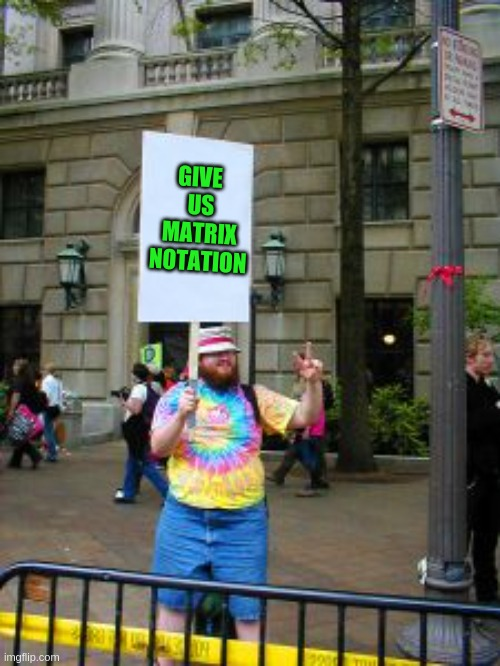
\includegraphics[width=0.3\textwidth]{img/meme_matrix-notation}
\end{center}

\end{frame}
}

\begin{frame}{The data in matrix form}

Let $\vec X$ represent the observations for all training points:

\begin{equation}
\vec X := 
\left(
\begin{array}{cccccc}
\Big| & \Big| & & \Big| & & \Big| \\[3mm]
\vec x^{(1)} & \vec x^{(2)} & \cdots & \vec x^{(\alpha)} & \cdots & \vec x^{(p)}\\[2mm]
\Big| & \Big| & & \Big| & & \Big|
\end{array}
\right) \in \R^{2 \times p}
\end{equation}

and let $\vec y_{\text{True}}$ represent the true labels for all training points:

\begin{equation}
\vec y_{\text{True}} := (y_T^{(1)}, \ldots, y_T^{(p)}) \in \R^{1 \times p}
\end{equation}

\end{frame}

\notesonly{
From this follows:
}

\begin{frame}{The qudaratic cost (MSE)}

\slidesonly{
    \vspace{-6mm}
    \hspace{8.cm}
    \StickyNote[1.5cm]{
        \begingroup
        \footnotesize
        \begin{equation}
        \vec X \in \R^{2 \times p}
        \end{equation}
        \begin{equation}
        \vec y_{\text{True}} \in \R^{1 \times p} 
        \end{equation}
        \begin{equation}
        \vec H := \frac{1}{p} \vec X~\vec X^\top
        \end{equation}
        \endgroup
    }[3cm]
    \vspace{-14mm}
}

\begin{align}
E^T_{\text{quadr.}}
    &= \frac{1}{2p} \big\lVert \vec w^\top \vec X - \vec y_{\text{True}} \big\rVert_2^2\\
    &= \frac{1}{2p} \underbrace{\left( \vec w^\top \vec X - \vec y_{\text{True}} \right)}_{1 \times p} \underbrace{\left( \vec w^\top \vec X - \vec y_{\text{True}} \right)^\top}_{p \times 1}
    \svspace{-3mm}
    \intertext{with $\vec y_{\text{True}} = \underline{\mathbf{w}}^{*\top}\vec X$:}
    &= \frac{1}{2p} \left( \vec w^\top \vec X - \vec \underline{\mathbf{w}}^{*\top} \vec X \right) \left( \vec w^\top \vec X - \vec \underline{\mathbf{w}}^{*\top} \vec X \right)^\top\\
\notesonly{
    &= \frac{1}{2p} \left( \vec w - \vec \underline{\mathbf{w}}^{*} \right)^\top \vec X \left(\left( \vec w^\top - \vec \underline{\mathbf{w}}^{*\top} \right) \vec X \right)^\top\\
\intertext{with $(\vec A~\vec B)^\top=\vec B^\top\vec A^\top$:}
    &= \frac{1}{2p} \left( \vec w - \vec \underline{\mathbf{w}}^{*} \right)^\top \vec X~\vec X^\top \left( \vec w^{\top} - \vec \underline{\mathbf{w}}^{*\top} \right)^\top\\
}
    &= \frac{1}{2p} \left( \vec w - \vec \underline{\mathbf{w}}^{*} \right)^\top \vec X~\vec X^\top \left( \vec w - \vec \underline{\mathbf{w}}^{*} \right)\\
    &= \frac{1}{2} \left( \vec w - \vec \underline{\mathbf{w}}^{*} \right)^\top \vec H \left( \vec w - \vec \underline{\mathbf{w}}^{*} \right)
\end{align}


\end{frame}

\begin{frame}{The gradient}

\slidesonly{
    \vspace{-15mm}
    \hspace{8.cm}
    \StickyNote[1.5cm]{
        \begingroup
        \footnotesize
        \begin{equation}
        \vec X \in \R^{2 \times p}
        \end{equation}
        \begin{equation}
        \vec y_{\text{True}} \in \R^{1 \times p} 
        \end{equation}
        \begin{equation}
        \vec H := \frac{1}{p} \vec X~\vec X^\top
        \end{equation}
        \endgroup
    }[3cm]
    \vspace{-14mm}
}

\begin{align}
\vec g
\;\;&=\;\;
\frac{1}{p} \sum_{\alpha=1}^{p} \;
\big( \vec x^{(\alpha)} \, \vec w^{\top}\vec x^{(\alpha)} - \vec x^{(\alpha)} y_{T}^{(\alpha)} \big)\\
\;\;&=\;\;
\frac{1}{p} \sum_{\alpha=1}^{p} \;
\big( \vec x^{(\alpha)} \, {\vec x^{(\alpha)}}^{\top} \vec w- \vec x^{(\alpha)} y_{T}^{(\alpha)} \big)\\
\;\;&=\;\;
\frac{1}{p} \left(\, \vec X \, \vec X^\top \vec w - \vec X\, \vec y_{\text{True}}^\top \right) =  \vec H~\vec w - \frac{1}{p} \vec X \vec y_{\text{True}}^\top
\end{align}

\end{frame}

\begin{frame}{The gradient}

\slidesonly{
\only<1>{
\begin{equation}
\vec g
\;\;=\;\;
\frac{1}{p} \left(\, \vec X \, \vec X^\top \vec w - \vec X\, \vec y_{\text{True}}^\top \right)
\end{equation}
}
}

stationary point:

\begin{align}
\only<1,2>{
\vec g \eqexcl \vec 0 \iff \vec X \, \vec X^\top \vec w^*  &= \vec X\, \vec y_{\text{True}}^\top\\
}
\vec w^* &=
{
\underbrace{
\left(
\vec X \, \vec X^\top
\right)
}_{\substack{\text{assumes}\\ \text{invertibility}}} 
}^{-1} \vec X\, \vec y_{\text{True}}^\top
\end{align}

$\vec w^*$ is a global minimum because\slidesonly{\only<1>{...?}}
\pause
\begin{enumerate}[1\notesonly{.}]
\item it is a unique solution of $\vec g = \vec 0$ and
\item 
\begin{equation}
\vec H 
= \frac{1}{p} \sum_{\alpha=1}^{p} \;
\vec x^{(\alpha)}~{\vec x^{(\alpha)}}^\top 
= \frac{1}{p} \, \vec X \, \vec X^\top = \vec C
\end{equation}
where $\vec C$ is the \emph{empirical covariance matrix} of centered data which is positive definite for invertible $\vec X\, \vec X^\top$.
\end{enumerate}

\pause
positive definiteness:
\begin{align}
\forall \vec z \in \R^2: \quad \vec z^\top \vec H\, \vec z 
\, &= \frac{1}{p} \, \vec z^\top \vec X \, \vec X^\top \vec z\notesonly{\\
\, &}= \frac{1}{p} \, \Big \lVert \, \vec X^\top \vec z \, \Big \rVert_2^2 > 0 \quad \mathrm{iff.} \; \vec z \ne \vec 0
\end{align}

\end{frame}

\subsection{Solution with regularization}

\begin{frame}

$L_2$ regularization cost:
\begin{equation}
E^R_{[\vec w]} := \frac{1}{2} \sum_{(i, j, v', v)} 
			\kern-2ex
			\big( \mathrm{w}_{ij}^{v'v} \big)^2 = \frac{1}{2} \lVert \vec w \rVert_2^2 = \frac{1}{2} \vec w^\top \vec w 
\end{equation}
\renewcommand{\CancelColor}{\color{gray}}
\begin{equation}
\frac{\partial}{\partial \vec w} E^R_{[\vec w]} = \slidesonly{\only<1>{...?}}\visible<2>{
\frac{1}{\wcancel{2}} \cdot \wcancel{2} \cdot \vec w = \vec w
}
\end{equation}
\pause
The regularized cost function:

\begin{equation}
	R_{[\vec{w}]} = \underbrace{ E_{[\vec{w}]}^T }_{
			\substack{\text{training} \\ \text{error} \\ \text{e.g. quadratic cost}}}
		+ \underbrace{ \lambda E_{[\vec{w}]}^R }_{
			\substack{\text{regularization} \\ \text{term}}}
		\eqexcl \min_{\vec w}
\end{equation}

where 
\begin{itemize}
	\item $E^R \; \corresponds \; $ prior knowledge of solution
	\item $\lambda:$ regularization parameter 
\end{itemize}
\end{frame}

\begin{frame}
Gradient:
\slidesonly{
\begin{equation*}
	R_{[\vec{w}]} = \underbrace{ E_{[\vec{w}]}^T }_{
			\substack{\text{training} \\ \text{error} \\ \text{e.g. quadratic cost}}}
		+ \underbrace{ \lambda E_{[\vec{w}]}^R }_{
			\substack{\text{regularization} \\ \text{term}}}
		\eqexcl \min_{\vec w}
\end{equation*}
}
\visible<1->{
\begin{align}
\vec g^R :=  \slidesonly{\only<1>{...?}}\visible<2>{\frac{\partial}{\partial \vec w} R_{[\vec w]}
&= \frac{\partial}{\partial \vec w} E^T_{[\vec w]} + \frac{\partial}{\partial \vec w} E^R_{[\vec w]}\\
&= \frac{1}{p} \left(\, \vec X \, \vec X^\top \vec w - \vec X\, \vec y_{\text{True}}^\top \right) + \vec I_N \, \lambda \, \vec w\\[2mm]
\iff& \quad \vec X \, \vec X^\top \vec w - \vec X\, \vec y_{\text{True}}^\top + p \lambda \, \vec I_N \,  \vec w \eqexcl \vec 0\\[2mm]
\vec w^* &=  {\underbrace{
\left(\, \vec X \, \vec X^\top + p \lambda \, \vec I_N \,  \right)
}_{
\substack{
\text{positive definite and}\\
\text{therefore invertible}\\
}
}
}^{-1} \vec X \, \vec y_{\mathrm{True}}^{\top}
}
\end{align}
}

\end{frame}
